\chapter{Model}
\paragraph{What Model Was Used}
The model used for this research was a Generalized Additive Model (GAM) with random intercepts.
To explain what a GAM with random intercepts is, we first have to introduce some lower-level models.\\
\section{From LM to GLM to GAM to GAM + re}
Linear regression is a method used to describe how the average 
value of a numerical outcome changes according to a linear 
combination of predictors.
This kind of regression can be used to represent relationships 
between variables.
However, the linear regression model relies on several strong assumptions, 
in particular that the response variable is continuous, 
normally distributed, and linearly related to the predictors. 
In many real-world applications, these assumptions are not appropriate. 
As in our case our outcome is non-normally distributed, we need
to use a different model.
\subsubsection{Linear Model (LM)}
\begin{equation}
Y_i = \beta_0 + \beta_1x_{i1} + \cdots + \beta_px_{ip} + \varepsilon_i,
\end{equation}

where

\begin{equation}
\varepsilon_i \sim N(0,\sigma^2).
\end{equation}

and:
\begin{itemize}
    \item $Y_i$ is the response variable;
    \item $\beta_0$ is the intercept;
    \item $\beta_1,\ldots,\beta_p$ are the regression coefficients associated with the predictors;
    \item $x_{i1},\ldots,x_{ip}$ are the values of the predictors for observation $i$;
    \item $\varepsilon_i$ is the random error term, assumed to be independently and identically distributed as
    \[
    \varepsilon_i \sim N(0,\sigma^2).
    \]
\end{itemize}\\
\small Source: \textcite[p.~37]{gelman2007book}

\subsection{From LM to GLM}
To address these above-mentioned limitations, we can resort to 
the Generalized Linear Model (GLM), which extends the classical
linear model by allowing the response variable to follow 
distributions from the exponential family and by introducing a 
link function that connects the expected value of the response 
to the linear predictor.
\subsubsection{Generalized Linear Model (GLM)}

\begin{equation}
g(\mu_i)=
\beta_0+\beta_1x_{i1}+\cdots+\beta_px_{ip},
\end{equation}

where

\begin{equation}
\mu_i=E(Y_i),
\end{equation}

and:
\begin{itemize}
    \item $\mu_i=E(Y_i)$ is the expected value of the response variable;
    \item $g(\cdot)$ is the link function;
    \item $\eta_i$ denotes the linear predictor.
\end{itemize}\\
\small Source: \textcite[p.~109]{gelman2007book}

\subsection{From GLM to GAM}
While GLMs provide a flexible framework for handling different
types of response variables, they still assume a linear 
relationship between the transformed expected value of the
response and the predictors. In practice, this assumption would
still be too restrictive, since many relationships in real 
data are non-linear.\\
To overcome this limitation, Generalized Additive Models (GAMs) 
extend GLMs by allowing the linear predictor to include smooth, 
functions of the covariates. This makes it possible to model 
complex and potentially non-linear effects of predictors on the 
response variable while maintaining interpretability.
\subsubsection{Generalized Additive Model (GAM)}

\begin{equation}
g(\mu_i)=
\beta_0+
f_1(x_{i1})+
f_2(x_{i2})+
\cdots+
f_p(x_{ip}) +
\varepsilon_i,
\end{equation}

where $f_j(\cdot)$ are smooth functions estimated from the data.\\
\small Source: \textcite[p.~307]{james2021islr}

\subsection{From GAM to GAM + re}
Although GAMs allow for flexible functional forms, standard models assume that 
all observations are independent. In our case, however, the data points are 
grouped by continent. Observations belonging to the same continent might share unobserved characteristics 
not captured by the other predictors, which could violate this assumption of 
independence.\\
To account for this shared structure, we included a random intercept for the 
continent variable directly within the GAM framework. In R, this is implemented 
using a random effect smooth basis (\texttt{bs = "re"}). This approach allows 
the model to estimate and control for baseline differences across continents, 
adjusting for the fact that data within the same continent may be correlated, 
while still accurately capturing the non-linear relationships of the other 
variables.

\subsubsection{Generalized Additive Model with Random Intercepts (GAM + re)}
\begin{equation}
g(\mu_i) = \beta_0 + \sum_{j=1}^{p}f_j(x_{ij}) + \mathbf{Z}_i\mathbf{b} + \varepsilon_i
\end{equation}
where:
\begin{itemize}
    \item $\mathbf{Z}_i$ is the design matrix row associated with the random effects;
    \item $\mathbf{b}$ is the vector of random effects, assumed to be normally distributed as $\mathbf{b} \sim N(\mathbf{0}, \mathbf{D})$.
\end{itemize}
In our specific formulation, $\mathbf{b}$ reduces to a single random intercept per 
continent, and the covariance matrix $\mathbf{D}$ simplifies to a single scalar 
variance component $\sigma^2_{\text{continent}}$, since no random slopes or nested 
grouping structures are included in the model.\\
\small Source: \textcite[p.~307]{james2021islr} for GAM model and \textcite[p.~105]{zuur2009mixed_effects_models} for the random-effects component $\mathbf{Z}_i\mathbf{b}$.


\subsection{Model Specification for This Study}
Initial models using a Gaussian family on the original scale 
yielded poor goodness-of-fit, with negative adjusted $R^2$ values. 
Given the positive and right-skewed distribution of video game 
sales, a Gamma family with log link was initially considered as 
a more appropriate distributional assumption \cite{hosch2026gamma}. 
However, applying a log transformation to the response variable 
substantially improved residual behaviour and approximated 
normality, making a Gaussian family with log transformed sales, 
the most appropriate specification for the final model:

\begin{equation}
Y_i^* = \log(Y_i) \sim N(\mu_i, \sigma^2)
\end{equation}

where $Y_i$ represents video game sales in millions and $Y_i^*$ 
is the log-transformed response used in the final model.

\subparagraph{Formula of the Chosen Model}
\begin{equation}
\begin{aligned}
Y_i^* = \beta_0 + f_1(IU_i) + f_2(Year_i, DR_i) + f_3(U_i) + \beta_1 \cdot GNI_i + b_{c(i)} + \varepsilon_i
\end{aligned}
\end{equation}

where:

\begin{itemize}
    \item $Y_i$ denotes sales (in millions) for observation $i$;

    \item $\beta_0$ is the intercept term;
    
    \item $f_1(IU_i)$ represents the smooth nonlinear effect of Internet Users;
    
    \item $f_2(Year_i,DR_i)$ represents a joint nonlinear effect of Year and Depression Rates, modelled using a tensor product smooth;
    
    \item $f_3(U_i)$ represents the smooth nonlinear effect of Unemployment;
    
    \item $\beta_1$ represents the linear effect of GNI per capita;
    
    \item $b_{c(i)}$ is a continent-specific random effect;
    
    \item $\varepsilon_i$ is the error term, assumed to follow a normal distribution with mean zero and variance $\sigma^2$, i.e.,
    $\varepsilon_i \sim N(0,\sigma^2)$.
\end{itemize}

Below (Figure \ref{fig:Log_Model}) are the graphs of residuals of the chosen model, so after the log transformation.\\
Residual plots for the model prior to the log transformation are provided in the Appendix B (Figure \ref{fig:Non_Log_Model}).

\begin{figure}[H]
    \centering
    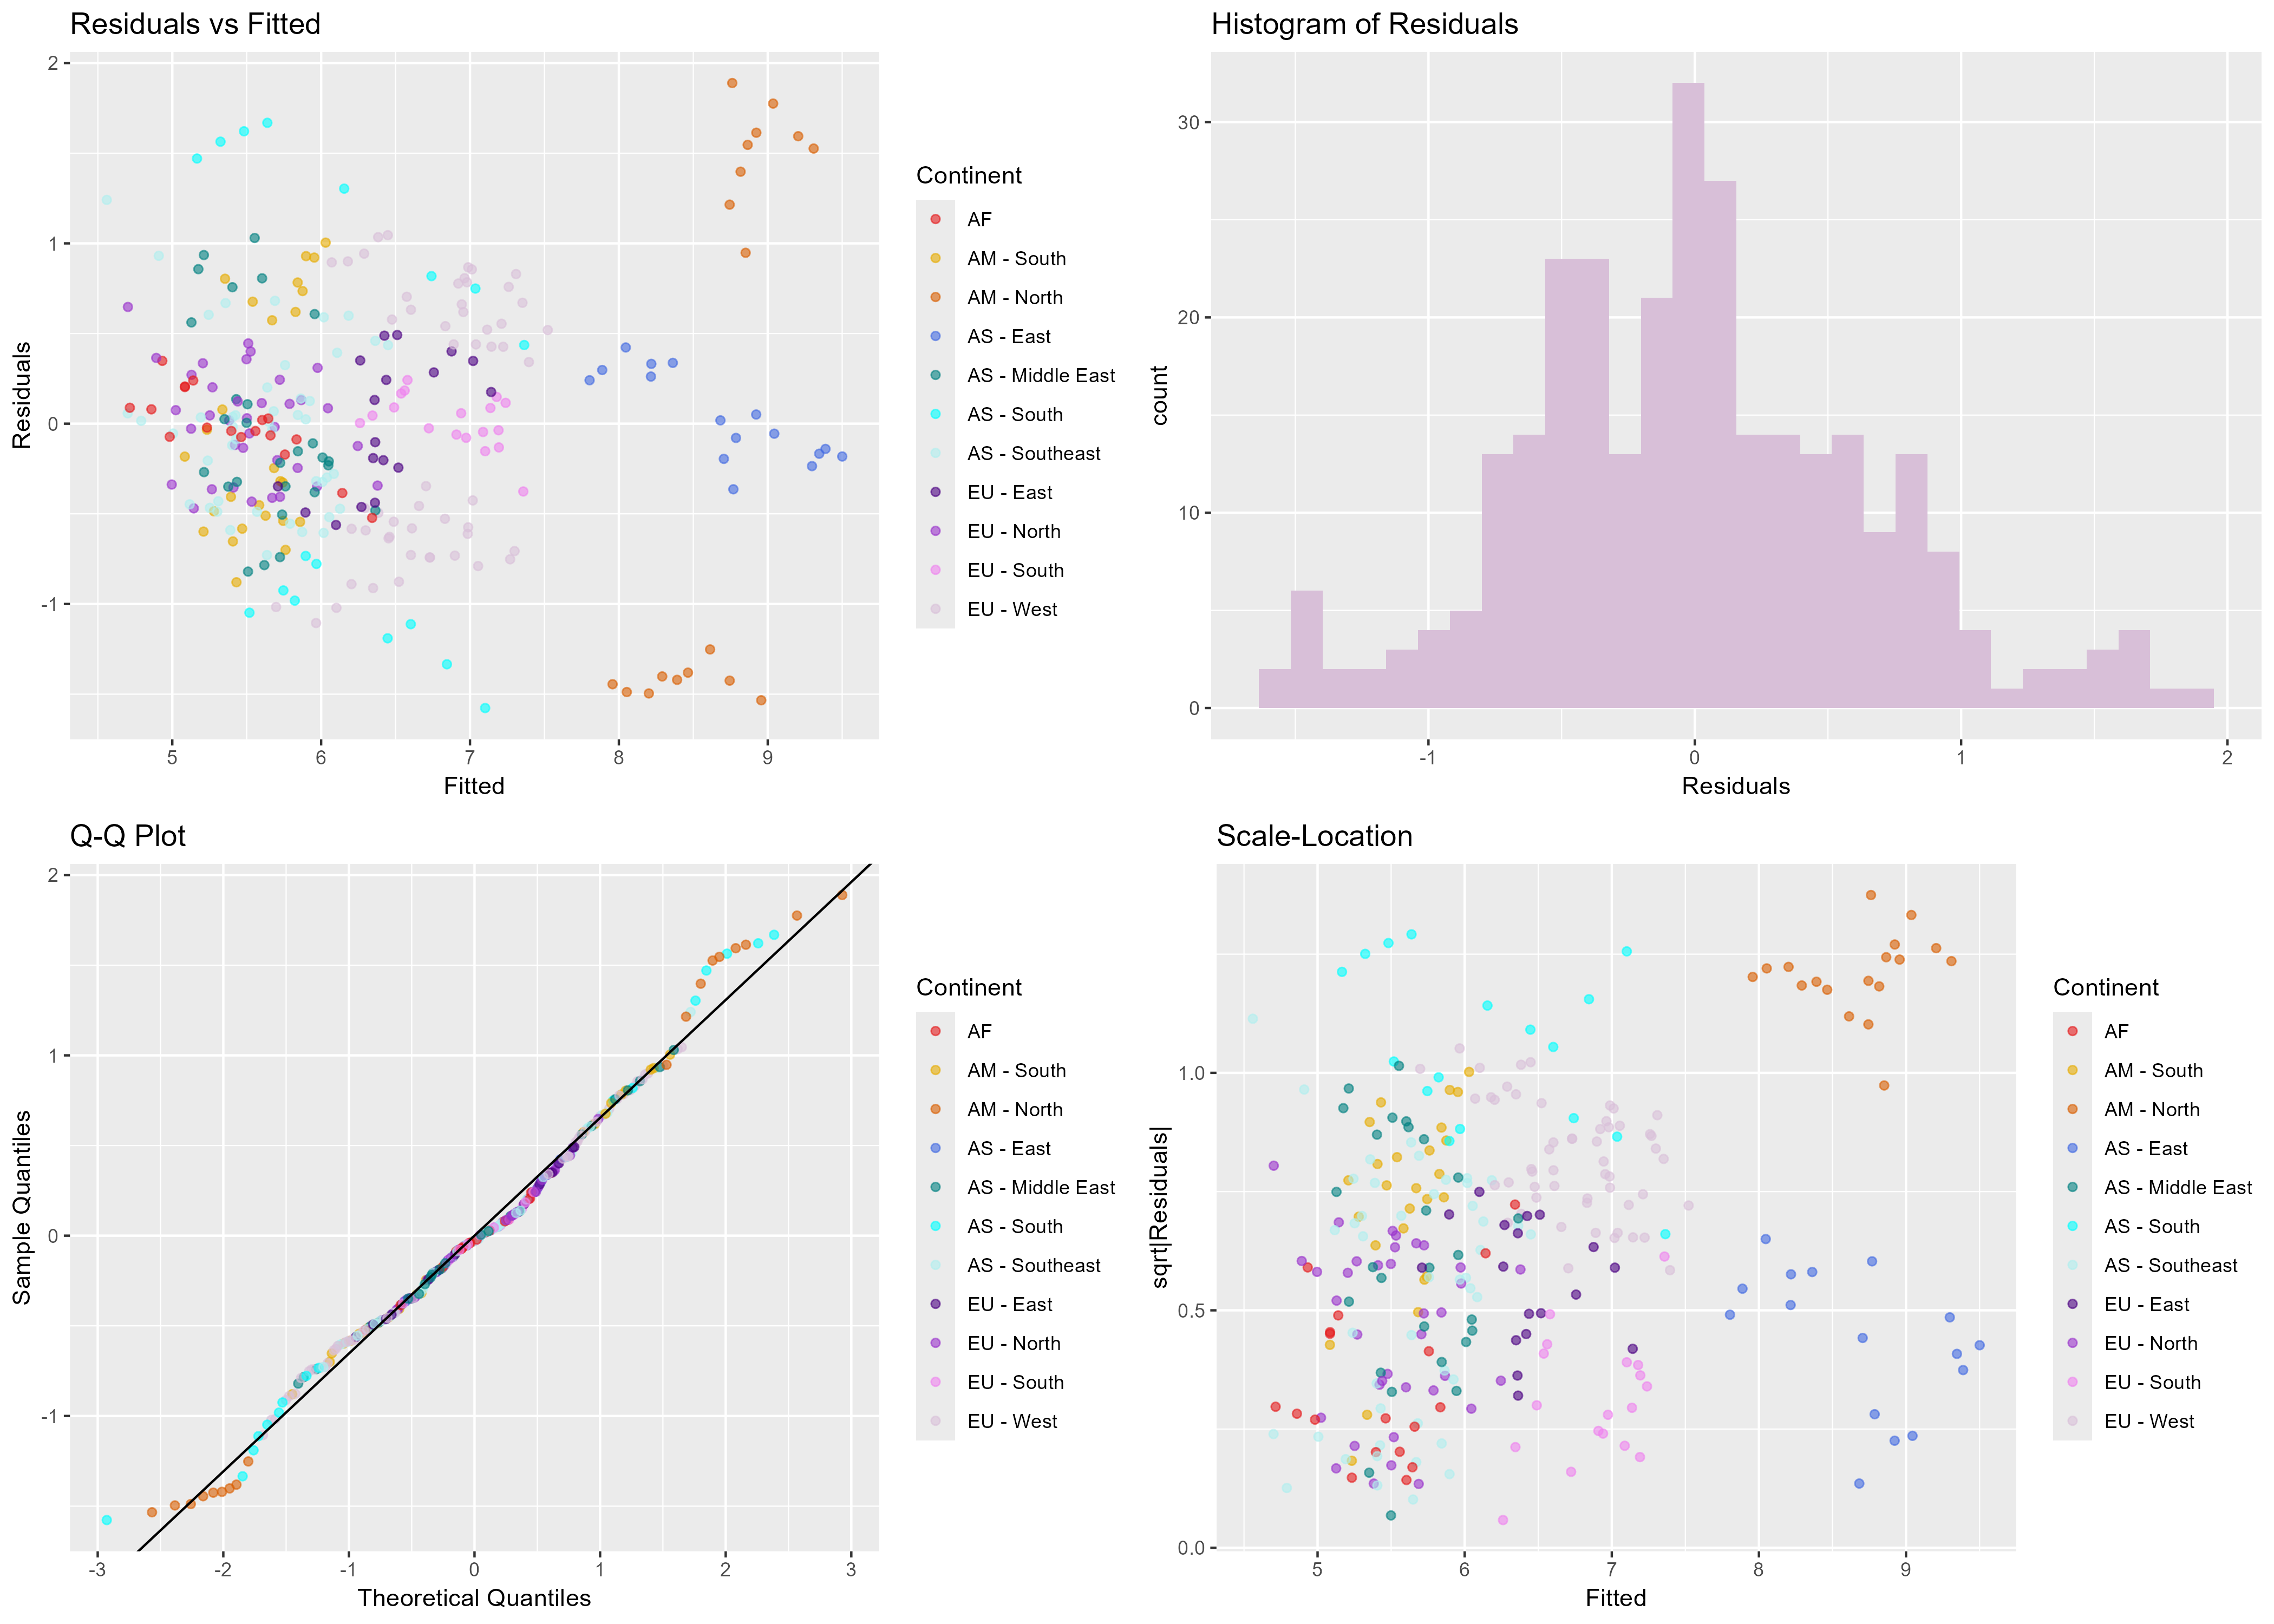
\includegraphics[width=\textwidth]{img/Log_Model_Colored_Graph.png}
    \caption{Diagnostic Residual Plots for the Log Model}
    \label{fig:Log_Model}
\end{figure}

\section{Model Results}
\begin{table}[H]
\centering
\caption{GAM + re Estimation Results}
\begin{tabular}{|l|c|c|c|c|}
\hline
\textbf{Variable} & \textbf{Estimate / edf} & \textbf{Std. Error / Ref.df} & \textbf{Statistic} & \textbf{p-value} \\
\hline\hline
\multicolumn{5}{|l|}{\textit{Parametric terms}} \\
\hline
Intercept & 6.860 & 0.417 & 16.469 & $<0.001^{***}$ \\
$GNI_i$ & $-1.072 \times 10^{-5}$ & $4.287 \times 10^{-6}$ & $-2.502$ & $0.013^{*}$ \\
\hline\hline
\multicolumn{5}{|l|}{\textit{Smooth terms}} \\
\hline
$f_1(IU_i)$ & 3.232 & 4.072 & 4.463 & $0.002^{**}$ \\
$f_2(Year_i,DR_i)$ & 6.522 & 6.898 & 10.261 & $<0.001^{***}$ \\
$f_3(U_i)$ & 2.346 & 2.977 & 4.736 & $0.003^{**}$ \\
$b_{c(i)}$ & 9.730 & 10.000 & 50.250 & $<0.001^{***}$ \\
\hline\hline
\multicolumn{5}{|l|}{\textit{Model fit}} \\
\hline
Adjusted $R^2$ & \multicolumn{4}{l|}{0.717} \\
Deviance explained & \multicolumn{4}{l|}{73.9\%} \\
REML & \multicolumn{4}{l|}{349.39} \\
$n$ & \multicolumn{4}{l|}{293} \\
\hline
\end{tabular}
\\[0.5em]
\small Significance codes: $^{***}p<0.001$, $^{**}p<0.01$, $^{*}p<0.05$
The complete R model specification is provided in Appendix C (Model \ref{lst:gam}).\\
Note: as it is possible to see, all the model's variables are
statistically significant. This is due to the fact that
non significant variables (e.g. Stringency Index), have been
removed in order to guarantee a parsimonious and efficient model.
\end{table}

The intercept is equal to 6.860, number that represents the 
baseline log sales value when all the other variables are equal
to 0.\\
GNI per Capita shows a linear and statistically significant negative effect 
on sales with an estimate of $-1.072 \times 10^{-5}$, 
suggesting that, all else being equal, higher national income 
is associated with slightly lower video game sales.
\begin{figure}[H]
    \centering
    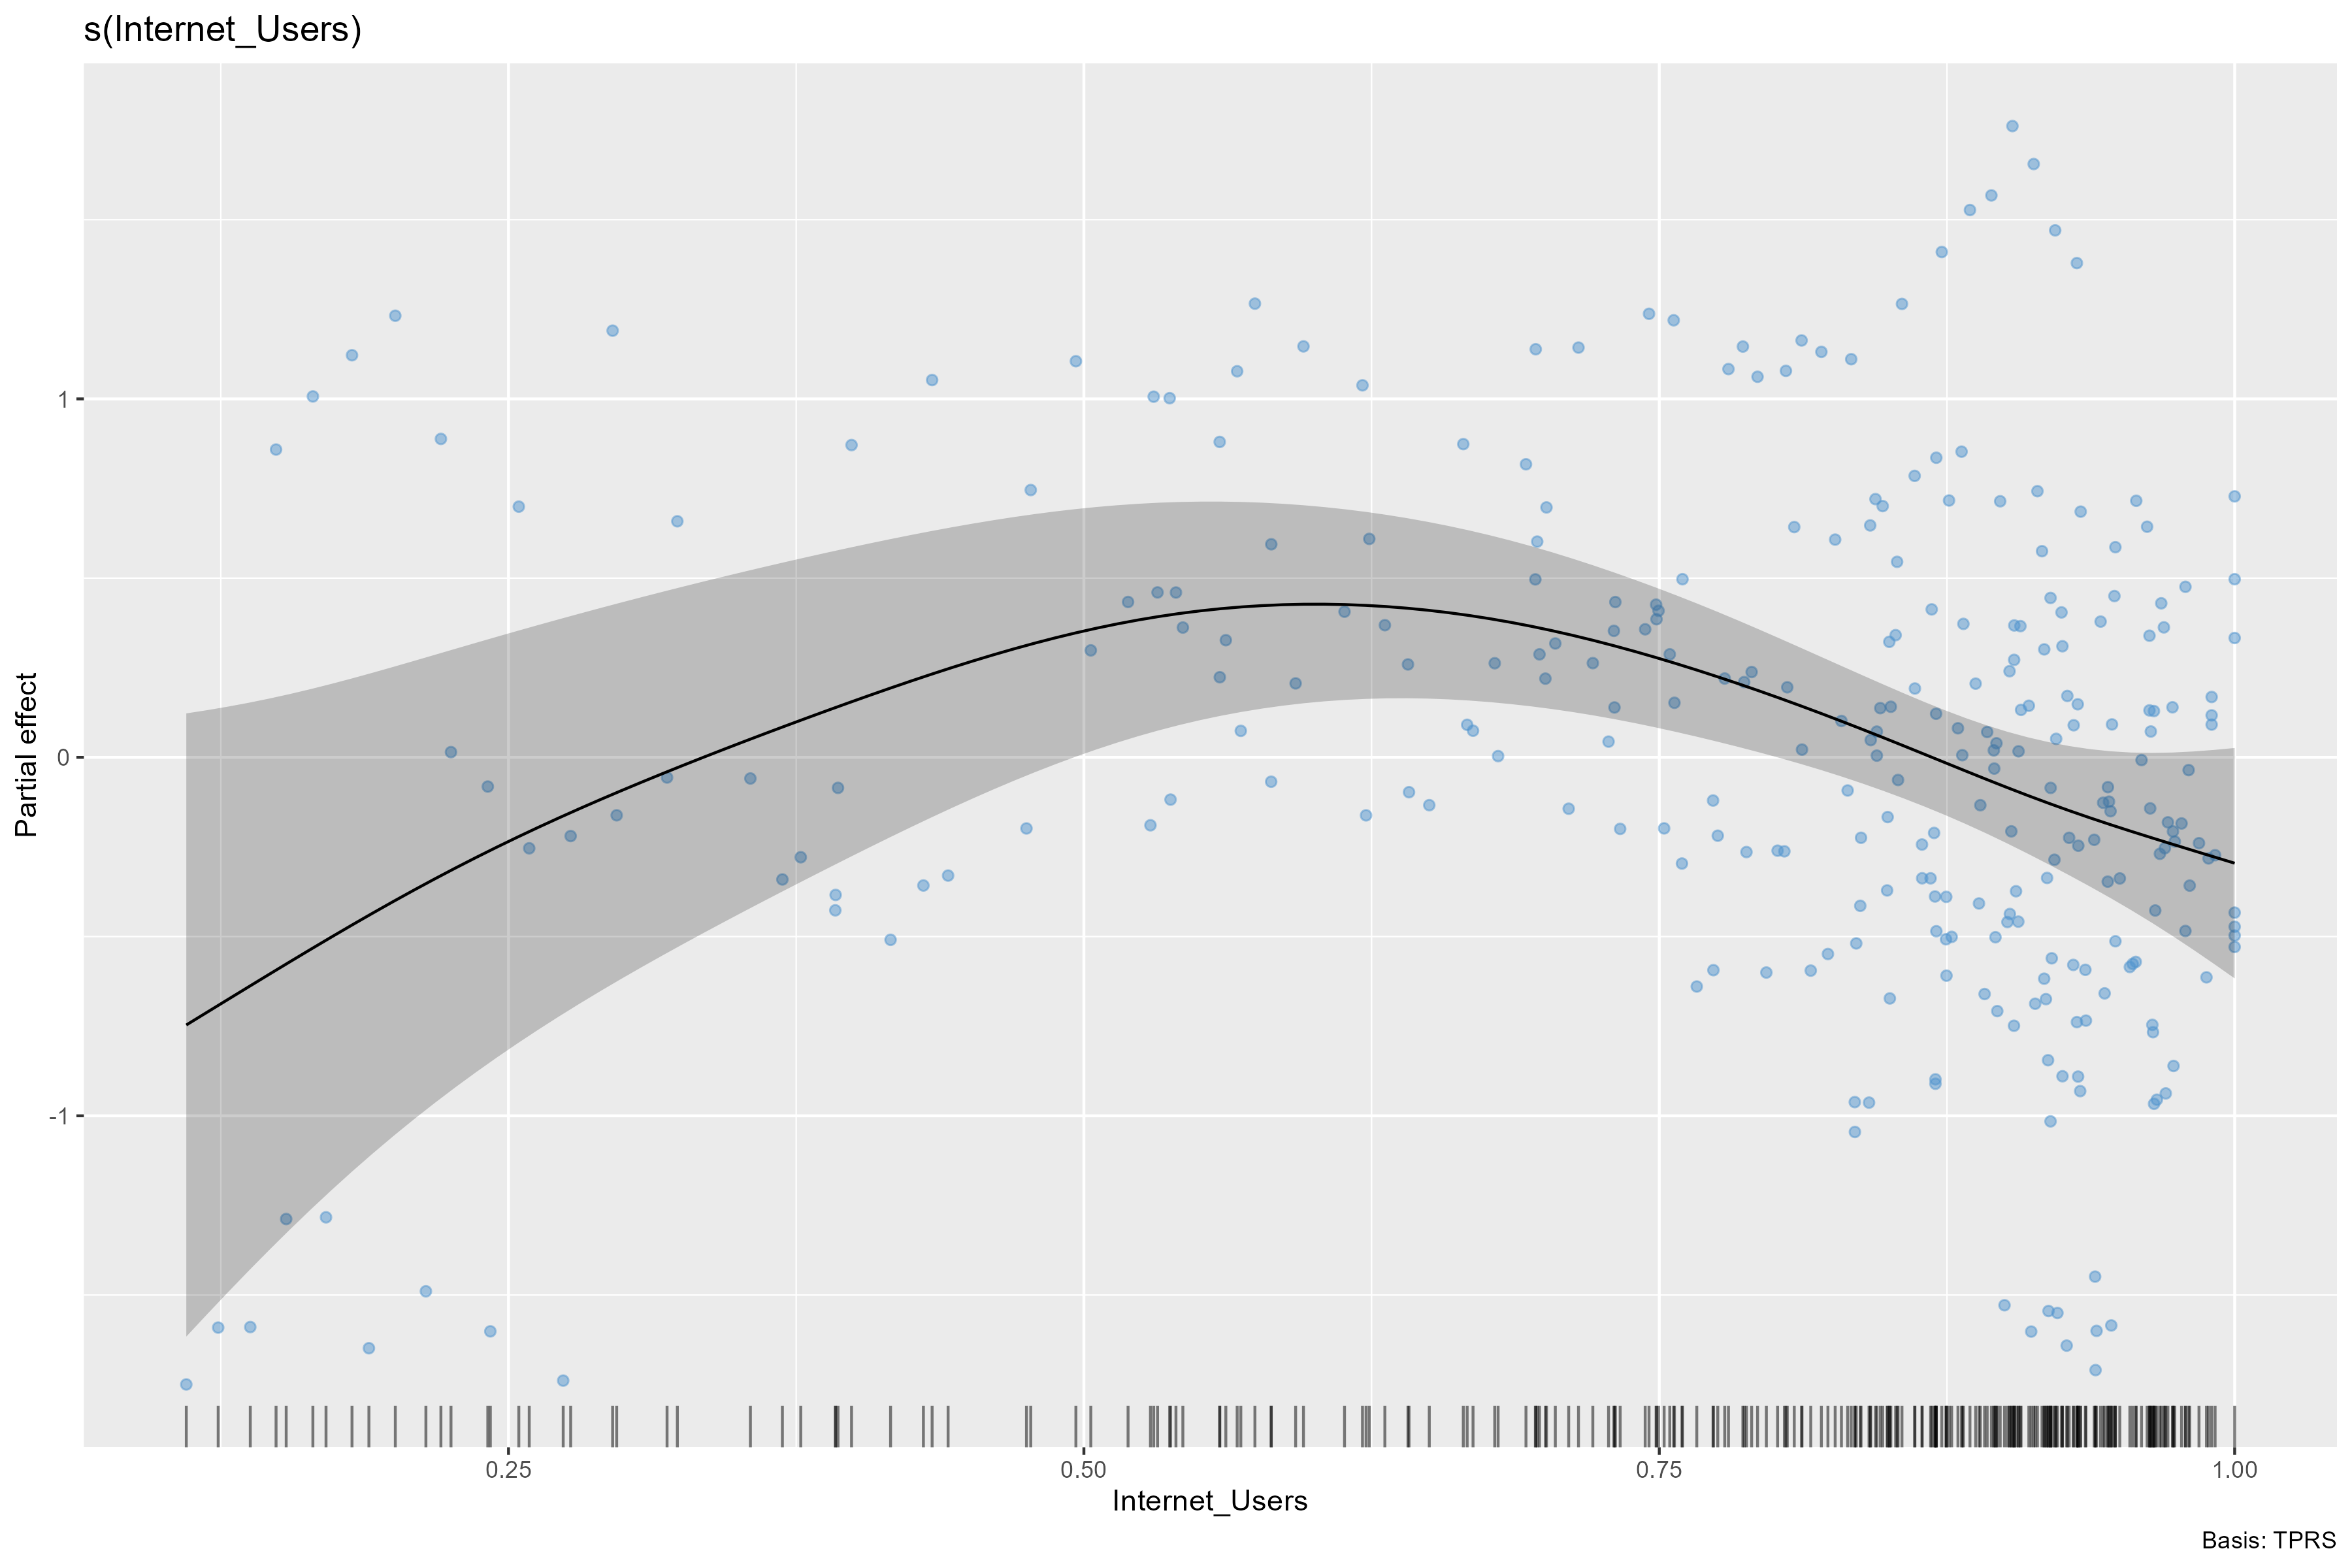
\includegraphics[width=\textwidth]{img/s_Internet_Users.png}
    \caption{Estimated partial effect of Internet Users on log(Sales)}
    \label{fig:s_Internet_Users}
\end{figure}
Internet Users exhibit a non-linear 
effect with an effective degrees of freedom (edf) value of 3.232 
suggesting a moderately flexible relationship (values of edf 
greater than 1 indicate nonlinear effects, with higher values 
reflecting greater functional flexibility).\\
While here the observations are more spread, the confidence 
interval is narrowest in the 0.75–1 range, where the rug plot 
confirms the highest concentration of observations, while it 
remains wide for the first three quarters of the spline where 
data are sparser.\\
A broader view shows that countries with 
intermediate internet penetration tend to be associated with 
higher sales in the video game market, while both less and more 
digitalized countries show a lower partial effect.\\
One possible explanation for the decline at high penetration rates is that 
in highly digitalized countries internet access extends across 
all age groups, including older demographics that may on average 
be less inclined to spend money on video games, though caution 
is needed in drawing causal conclusions from an observational 
model.
\begin{figure}[H]
    \centering
    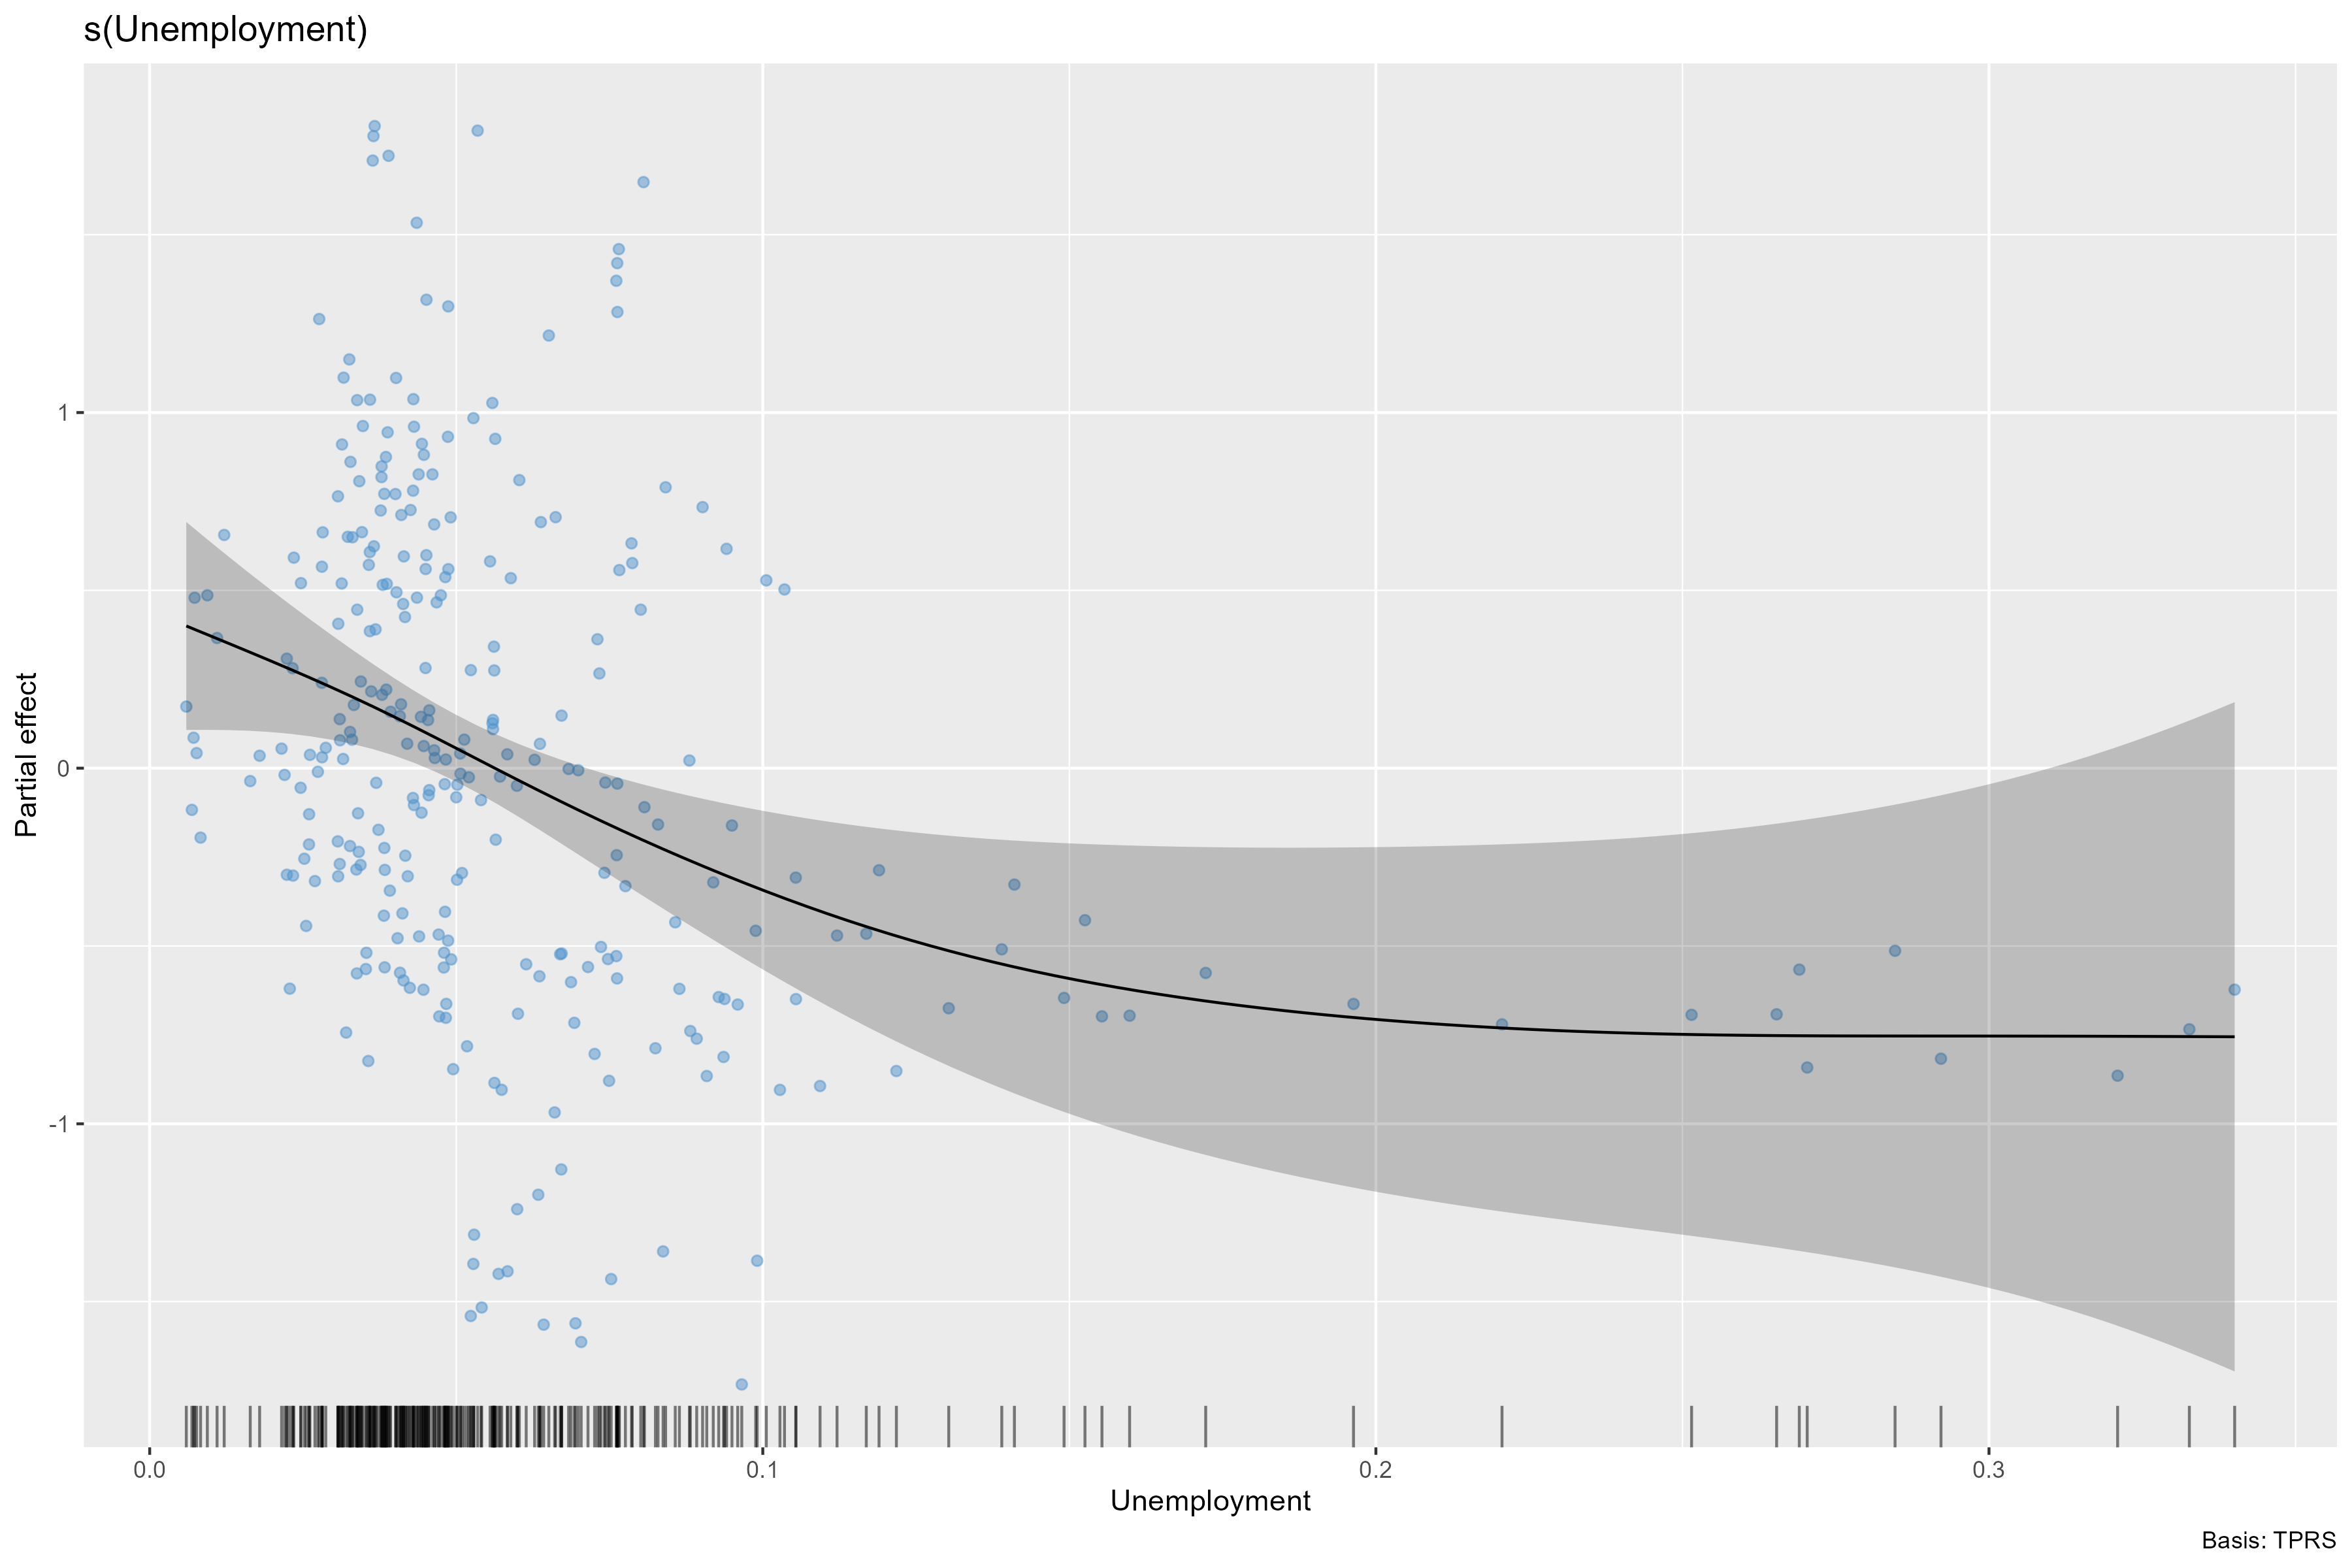
\includegraphics[width=\textwidth]{img/s_Unemployment.png}
    \caption{Estimated partial effect of Unemployment Rates on log(Sales)}
    \label{fig:s_Unemployment}
\end{figure}
Similarly, Unemployment displays a similar pattern, with an edf of 2.346
indicating a moderately flexible non-linear trend.\\
Unemployment's effect on our response variable (log(Sales)) 
starts from positive values when unemployment is near 0 and goes 
decreasing as unemployment increases.\\
It is important to notice 
that, as the vast majority of the observations are concentrated 
in a small range (0–0.1), this interval is the one with more 
statistical evidence of the effect (having a narrower confidence 
interval), while there are too few observations of unemployment 
values higher than 0.1, leading us to be more skeptical about 
the spline in that part.\\
Note that these represent partial 
effects, meaning all other variables in the model are held 
constant.
\begin{figure}[H]
    \centering
    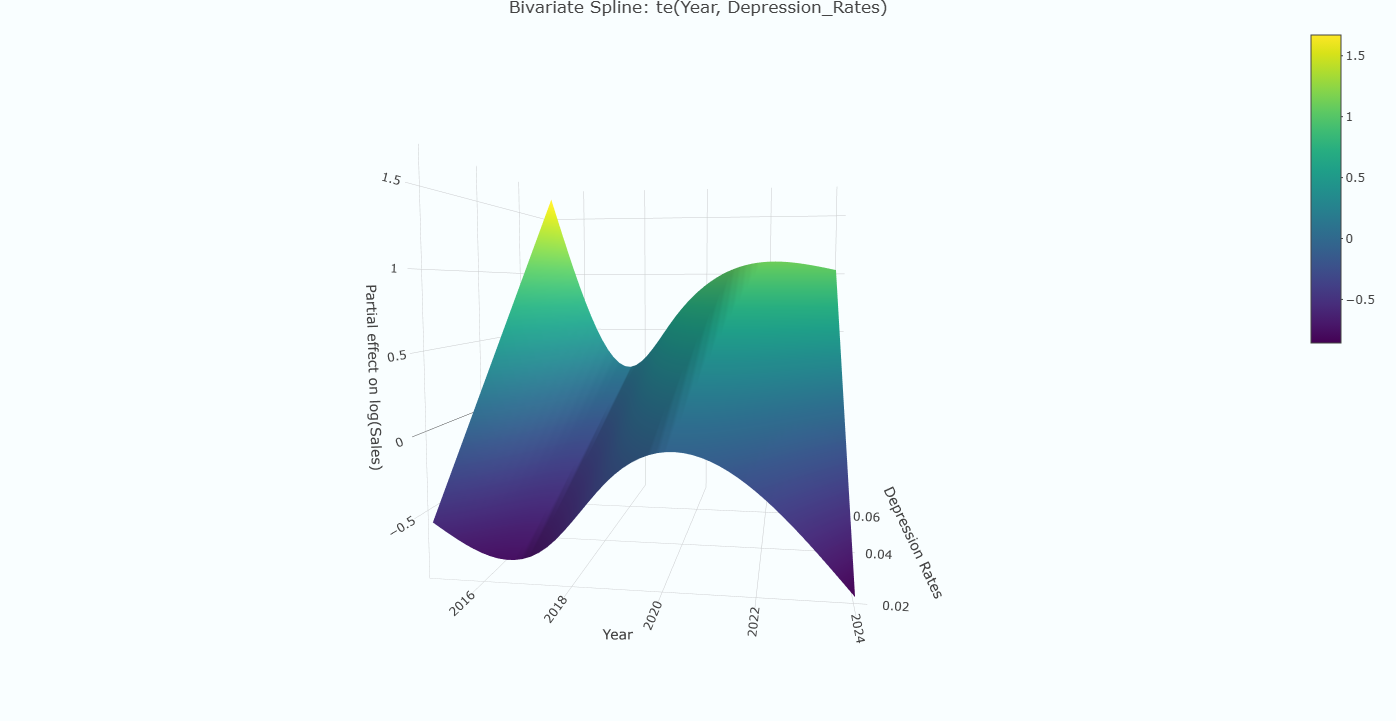
\includegraphics[width=\textwidth]{img/3D_Plot.png}
    \caption{3D visualization of the partial effect of $f_2(Year_i,DR_i)$ on log(Sales)}
    \label{fig:3D_Plot}
\end{figure}
The tensor product between Year and Depression Rates shows --
with an edf of 6.522 -- a strongly non linear and complex effect
of depression rates over sales, that is not constant over the years.\\
Overall, across all years, low depression rates are associated with lower sales, while higher 
depression rates tend to be associated with higher sales; even if it is important to remember that this refers to the 
partial effect, meaning all other variables in the model are held constant.\\
However, in the 2019–2022 period we can notice how depression rates start to have a stronger 
influence on the response variable, which could reflect a real-world effect tied to COVID-19:
rising depression rates coinciding with a boom in video games sales.
As for the spike around 2015-2016 at high depression rates, this is likely due to the scarcity 
of observations in that region of the data: where data points are few, the spline tends to 
behave in an unstable manner, producing estimates that are less reliable. This period should therefore be interpreted with caution.
\begin{figure}[H]
    \centering
    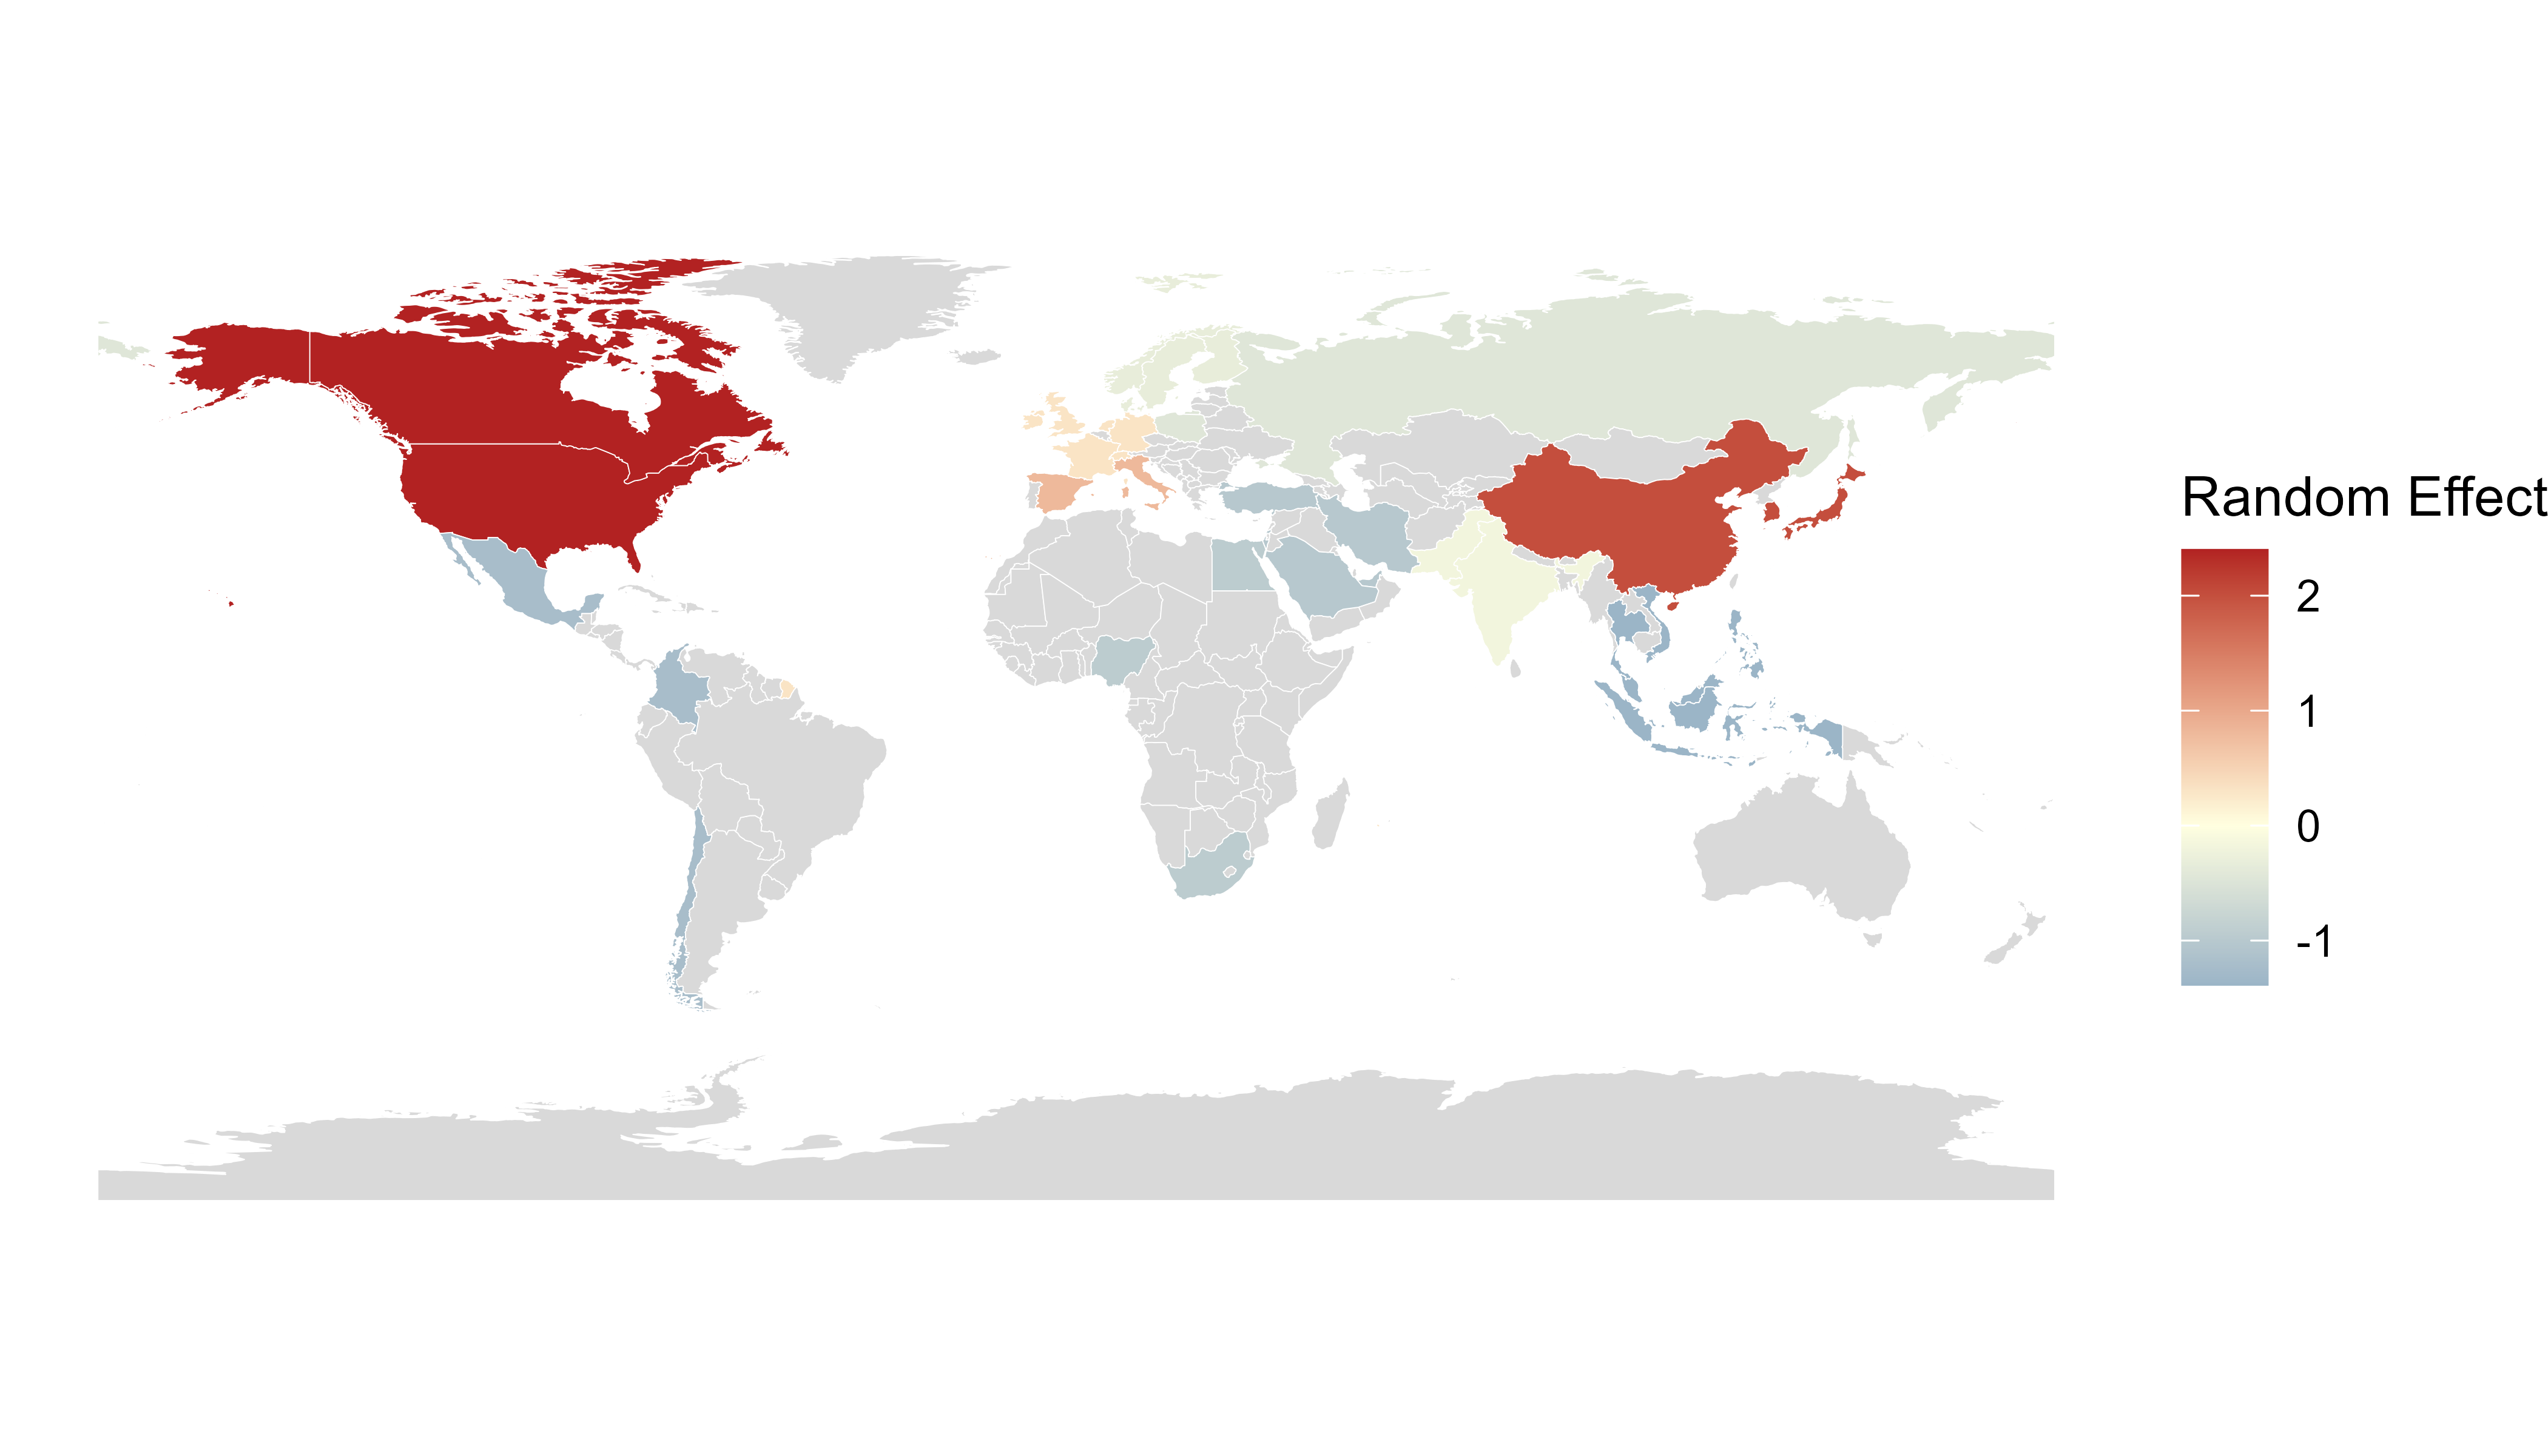
\includegraphics[width=\textwidth]{img/Random_Effect_Map.png}
    \caption{Random Effect Global Map}
    \label{fig:Random_Effect_Map}
\end{figure}
To conclude, to better illustrate the regional heterogeneity captured 
by the Continent term, the map visualizes the random effects estimated by the s(Continent, bs="re") term, capturing the residual variability in video game sales attributable to geographic location after accounting for all other covariates in the model. Countries shown in red exhibit systematically higher sales than what the other variables alone would predict, while countries in blue show the opposite pattern, and grey countries are absent from the dataset.
The most positive random effects are concentrated in North America and East Asia, which represent the world's historically dominant video game markets. Western Europe displays moderate positive effects, while Russia and Northern Europe show slight negative deviations.
The high edf of 9.730 for this term, approaching the maximum of 10, confirms the substantial regional heterogeneity captured by the model, with geography playing a meaningful role beyond what the continuous predictors can explain.
In general, the results indicate a strong overall fit, with an adjusted 
R-squared of 0.717 and a deviance explained of 73.9\%, 
suggesting that the model captures a substantial portion of the 
variability in sales.